\documentclass[11pt,a4paper]{article}

\usepackage[utf8]{inputenc}
\usepackage[margin=2.5cm]{geometry}
\usepackage{amsmath,amssymb}
\usepackage{graphicx}
\usepackage{booktabs}
\usepackage{hyperref}
\usepackage{xcolor}

\hypersetup{
    colorlinks=true,
    linkcolor=blue!70!black,
    citecolor=blue!70!black,
    urlcolor=blue!70!black
}

\title{\textbf{Empirical Study of Matrix Multiplication:\\Parallel Execution and Shared-Memory Scalability}}
\author{\textbf{Manuel Muñoz Roca} \\
Grado en Ciencia e Ingeniería de Datos \\
Universidad de Las Palmas de Gran Canaria (ULPGC) \\
\vspace{0.15cm}
\small \textbf{Repository:} \href{https://github.com/maneloco/BD-Individual-Assignment-3}{\texttt{github.com/maneloco/BD-Individual-Assignment-3}}}
\date{\today}

\begin{document}

\maketitle

\begin{abstract}
In this third assignment, I study the performance, speedup, and memory usage of shared-memory parallel matrix multiplication in C using POSIX Threads (\texttt{pthreads}). I use the loop-reordered $ikj$ algorithm from my second assignment as an equivalent sequential baseline. To avoid the overhead of creating and destroying threads on every multiplication, I implemented a simple, persistent thread pool using a circular task queue, mutexes, and condition variables.

I conducted controlled experiments on an Intel Core i5-12500H processor (12 physical cores and 16 logical threads) across 17 matrix sizes from $n = 1$ to $n = 4096$, and thread counts from 1 to 32. Each trial ran in an isolated child process using \texttt{fork()} with nanosecond monotonic timers and peak resident memory (RSS) tracking.

The results show that parallel execution only helps when the matrix is large enough. For small matrices ($n \le 128$), multithreading is actually slower than sequential execution because managing threads and locks takes longer than the multiplication itself. For large matrices ($n = 4096$), 16 threads achieve a speedup of \textbf{5.19$\times$}, reducing runtime from 25.30 seconds down to 4.88 seconds. Finally, running 24 and 32 threads shows a clear oversubscription penalty, where performance drops and runtime almost doubles due to operating system context switches and CPU cache thrashing.
\end{abstract}

\section{Introduction and Objectives}

Matrix multiplication is a fundamental operation in data science, used in linear algebra, covariance matrix calculations, and deep learning. Multiplying two square matrices of size $n \times n$ requires $2n^3$ arithmetic operations, giving it a cubic time complexity of $\mathcal{O}(n^3)$.

In Assignment 2, I optimized single-core execution by reordering loops ($ikj$) and applying cache blocking. However, modern CPUs do not get faster simply by increasing clock speeds; instead, they include multiple physical cores that can work in parallel. The natural next step to improve performance is shared-memory multithreading.

In theory, using $p$ threads could speed up the computation by up to $p$ times ($S(p) = p$). In practice, several physical bottlenecks prevent ideal scaling:
\begin{itemize}
    \item \textbf{Amdahl's Law:} Serial sections (such as assigning tasks, locking mutexes, and waiting at barriers) limit the maximum speedup.
    \item \textbf{Memory Bandwidth:} All CPU cores share the same memory bus to access RAM. When multiple threads stream data at the same time, memory bandwidth becomes saturated.
    \item \textbf{Core Heterogeneity:} The Intel Alder Lake architecture has high-performance cores (P-cores) with hyperthreading and smaller energy-efficient cores (E-cores), so not all threads compute at the same speed.
    \item \textbf{Oversubscription:} Running more software threads than physical CPU contexts forces the operating system to constantly pause and switch threads (context switching), which wastes time and evicts data from the CPU cache.
\end{itemize}

The main objective of this study is to measure how thread count and matrix size affect performance in a shared-memory system. Specifically, I focus on answering the following research questions:

\begin{itemize}
    \item \textbf{RQ1 (Speedup and Problem Size):} At what matrix dimension $n$ does parallel execution start beating the sequential baseline, and what speedup is achieved up to $n = 4096$?
    \item \textbf{RQ2 (Single-Thread Overhead):} What is the overhead of running the thread pool with only 1 thread compared to pure sequential code ($T_{\text{par}}(1) / T_{\text{seq}}$)?
    \item \textbf{RQ3 (Hardware Limits and Oversubscription):} How does performance scale when moving from physical cores ($p \le 12$) to logical threads ($p = 16$), and what happens when we oversubscribe the CPU with 24 and 32 threads?
    \item \textbf{RQ4 (Memory Usage and Cache Locality):} Does multithreading increase peak memory usage (Peak RSS), and does row partitioning prevent false sharing in the CPU cache?
\end{itemize}

\section{Algorithmic Design and Implementation}

\subsection{Equivalent Sequential Baseline (\texttt{ikj})}
The assignment requires comparing the parallel implementation against an \textit{equivalent} sequential baseline using the same algorithm, data layout, and precision.

In Assignment 2, I demonstrated that loop reordering ($ikj$) is the fastest dense implementation. In C, matrices are stored in row-major order (\texttt{data[i * n + j]}). In the naive \texttt{ijk} order, the inner loop accesses matrix $B$ by columns, jumping across memory and causing frequent cache misses. In \texttt{ikj} order:
\begin{itemize}
    \item $A[i][k]$ stays in a CPU register during the inner loop.
    \item $B[k][j]$ and $C[i][j]$ are accessed sequentially in memory (stride-1).
    \item With \texttt{-O3 -march=native}, the compiler automatically vectorizes the loop with AVX2 instructions, computing 4 doubles per cycle.
\end{itemize}
I use this exact sequential \texttt{ikj} kernel as the baseline for all comparisons.

\subsection{POSIX Thread Pool Architecture}
Calling \texttt{pthread\_create()} and \texttt{pthread\_join()} inside the timed multiplication adds 20 to 50 microseconds of overhead per thread, which would distort measurements for small matrices.

To avoid this, I built a persistent \textbf{POSIX Thread Pool} (\texttt{thread.h} and \texttt{thread.c}):
\begin{itemize}
    \item \textbf{Worker Threads:} The pool creates $p$ worker threads once at initialization. These threads stay alive during the entire benchmark run.
    \item \textbf{Circular Task Queue:} Tasks are queued in a FIFO ring-buffer, each containing a function pointer and an argument pointer (\texttt{void (*function)(void *arg)}).
    \item \textbf{Synchronization:} A single mutex (\texttt{pthread\_mutex\_t lock}) protects the queue. A condition variable (\texttt{has\_work}) wakes up workers when a task is submitted, and another (\texttt{all\_idle}) signals the main thread when all tasks are complete.
    \item \textbf{Deadlock Prevention:} Only one mutex is used (preventing circular lock dependencies), the lock is released \textit{before} executing the multiplication task, and condition waits are wrapped in \texttt{while} loops to handle spurious wakeups.
    \item \textbf{Barrier (\texttt{threadpool\_wait}):} Blocks the caller until all queued tasks are finished and all workers are idle.
\end{itemize}

\subsection{Work Partitioning and False Sharing}
To parallelize the multiplication, I divide the outer loop ($i$) among the worker threads in the pool (\texttt{parallel\_matmul.c}):
\begin{itemize}
    \item \textbf{Row Slicing:} Each thread receives a contiguous slice of rows $[\text{start\_row}, \text{end\_row})$. If $n$ is not divisible by $p$, the remainder is distributed by giving one extra row to the first threads ($\lfloor n / p \rfloor + (t < n\%p ? 1 : 0)$).
    \item \textbf{Zero False Sharing:} Each thread writes only to its assigned rows in matrix $C$. Because one row of doubles for $n \ge 8$ takes 64 bytes or more (a full cache line), threads never write to the same cache line, avoiding false sharing without any mutexes during the math.
    \item \textbf{Pointer Aliasing (\texttt{restrict}):} I declare data pointers using C99 \texttt{restrict} (\texttt{const double * restrict a\_data}, etc.), informing GCC that memory regions do not overlap so it can safely auto-vectorize the inner loop.
\end{itemize}

\section{Experimental Setup and Methodology}

\subsection{Hardware and Software Environment}
All tests were run natively on my laptop under controlled conditions. Table~\ref{tab:hardware} summarizes the machine specifications.

\begin{table}[h!]
\centering
\small
\begin{tabular}{ll}
\toprule
\textbf{Component} & \textbf{Specification} \\
\midrule
Processor & 12th Gen Intel(R) Core(TM) i5-12500H \\
Microarchitecture & Alder Lake (4 Performance-cores + 8 Efficient-cores) \\
Physical Cores & 12 cores \\
Logical Processors & 16 threads (P-cores support HyperThreading) \\
L1d Cache (Data) & 48 KiB per P-core / 32 KiB per E-core (448 KiB total) \\
L2 Cache & 1.25 MiB per P-core / 2 MiB per E-core cluster (9 MiB total) \\
L3 Cache (Shared) & 18 MiB shared \\
System RAM & 16 GiB DDR (15 GiB usable, 0 swap) \\
Operating System & Arch Linux (x86\_64, Kernel \texttt{6.12.7}) \\
Compiler & GCC 14.2.1 (\texttt{-std=c11}) \\
\bottomrule
\end{tabular}
\caption{Hardware and software experimental environment.}
\label{tab:hardware}
\end{table}

\subsection{Compilation Flags and Correctness}
The source code was compiled using GCC with the following optimization flags:
\begin{quote}
\texttt{-std=c11 -Wall -Wextra -Wpedantic -O3 -march=native -lpthread -lm}
\end{quote}
The flag \texttt{-O3} enables aggressive loop optimizations and auto-vectorization, while \texttt{-march=native} instructs GCC to use instructions supported by my Alder Lake processor (AVX2 and FMA).

I deliberately excluded \texttt{-ffast-math} to maintain strict IEEE 754 floating-point compliance, ensuring numbers are not reordered or rounded unsafely.

Before benchmarking, I verified numerical correctness by comparing the parallel output against the sequential baseline across all matrix sizes and thread counts using an automated test suite (\texttt{make run\_tests}). All tests passed with zero numerical differences.

\subsection{Benchmarking Protocol and Process Isolation}
To ensure fair and reproducible measurements:
\begin{enumerate}
    \item \textbf{Timing Boundary:} The timer measures only the matrix multiplication. Allocation and matrix initialization are done outside the timed block.
    \item \textbf{High-Resolution Timer:} I used \texttt{clock\_gettime(CLOCK\_MONOTONIC)}, which provides nanosecond precision and is immune to system clock changes.
    \item \textbf{Warm-up and Repetitions:} Before recording, I run an unrecorded warm-up trial (\texttt{rep = -1}) to prime CPU caches and OS page tables. Then, I record 5 repetitions and use the median to filter out operating system background noise.
    \item \textbf{Process Isolation with \texttt{fork()}:} On Linux, \texttt{getrusage()} reports the historical peak memory of a process, which never decreases even after calling \texttt{free()}. To ensure large tests do not affect smaller ones, every single trial runs in a separate child process via \texttt{fork()}.
    \item \textbf{Checksums:} After each run, I sum all elements of matrix $C$ to confirm that sequential and parallel versions produce identical results and to stop the compiler from eliminating the loop.
\end{enumerate}

\subsection{Parameter Space}
I evaluated 17 matrix sizes: powers of two from $n = 1$ to $512$, followed by increments of $+512$ up to $4096$ ($n \in \{1, 2, 4, 8, 16, 32, 64, 128, 256, 512, 1024, 1536, 2048, 2560, 3072, 3584, 4096\}$). 
Thread counts were varied across $p \in \{1, 2, 4, 8, 12, 16, 24, 32\}$, covering single-thread overhead, core scaling, and oversubscription.

\section{Experimental Results and Analysis}

All reported numbers represent the median of 5 independent repetitions.

\subsection{Speedup and Strong Scaling (RQ1)}
Figure~\ref{fig:speedup} shows the speedup $S(p) = T_{\text{seq}} / T_p$ across thread counts compared to the ideal linear line ($S = p$).

\begin{figure}[htbp]
\centering
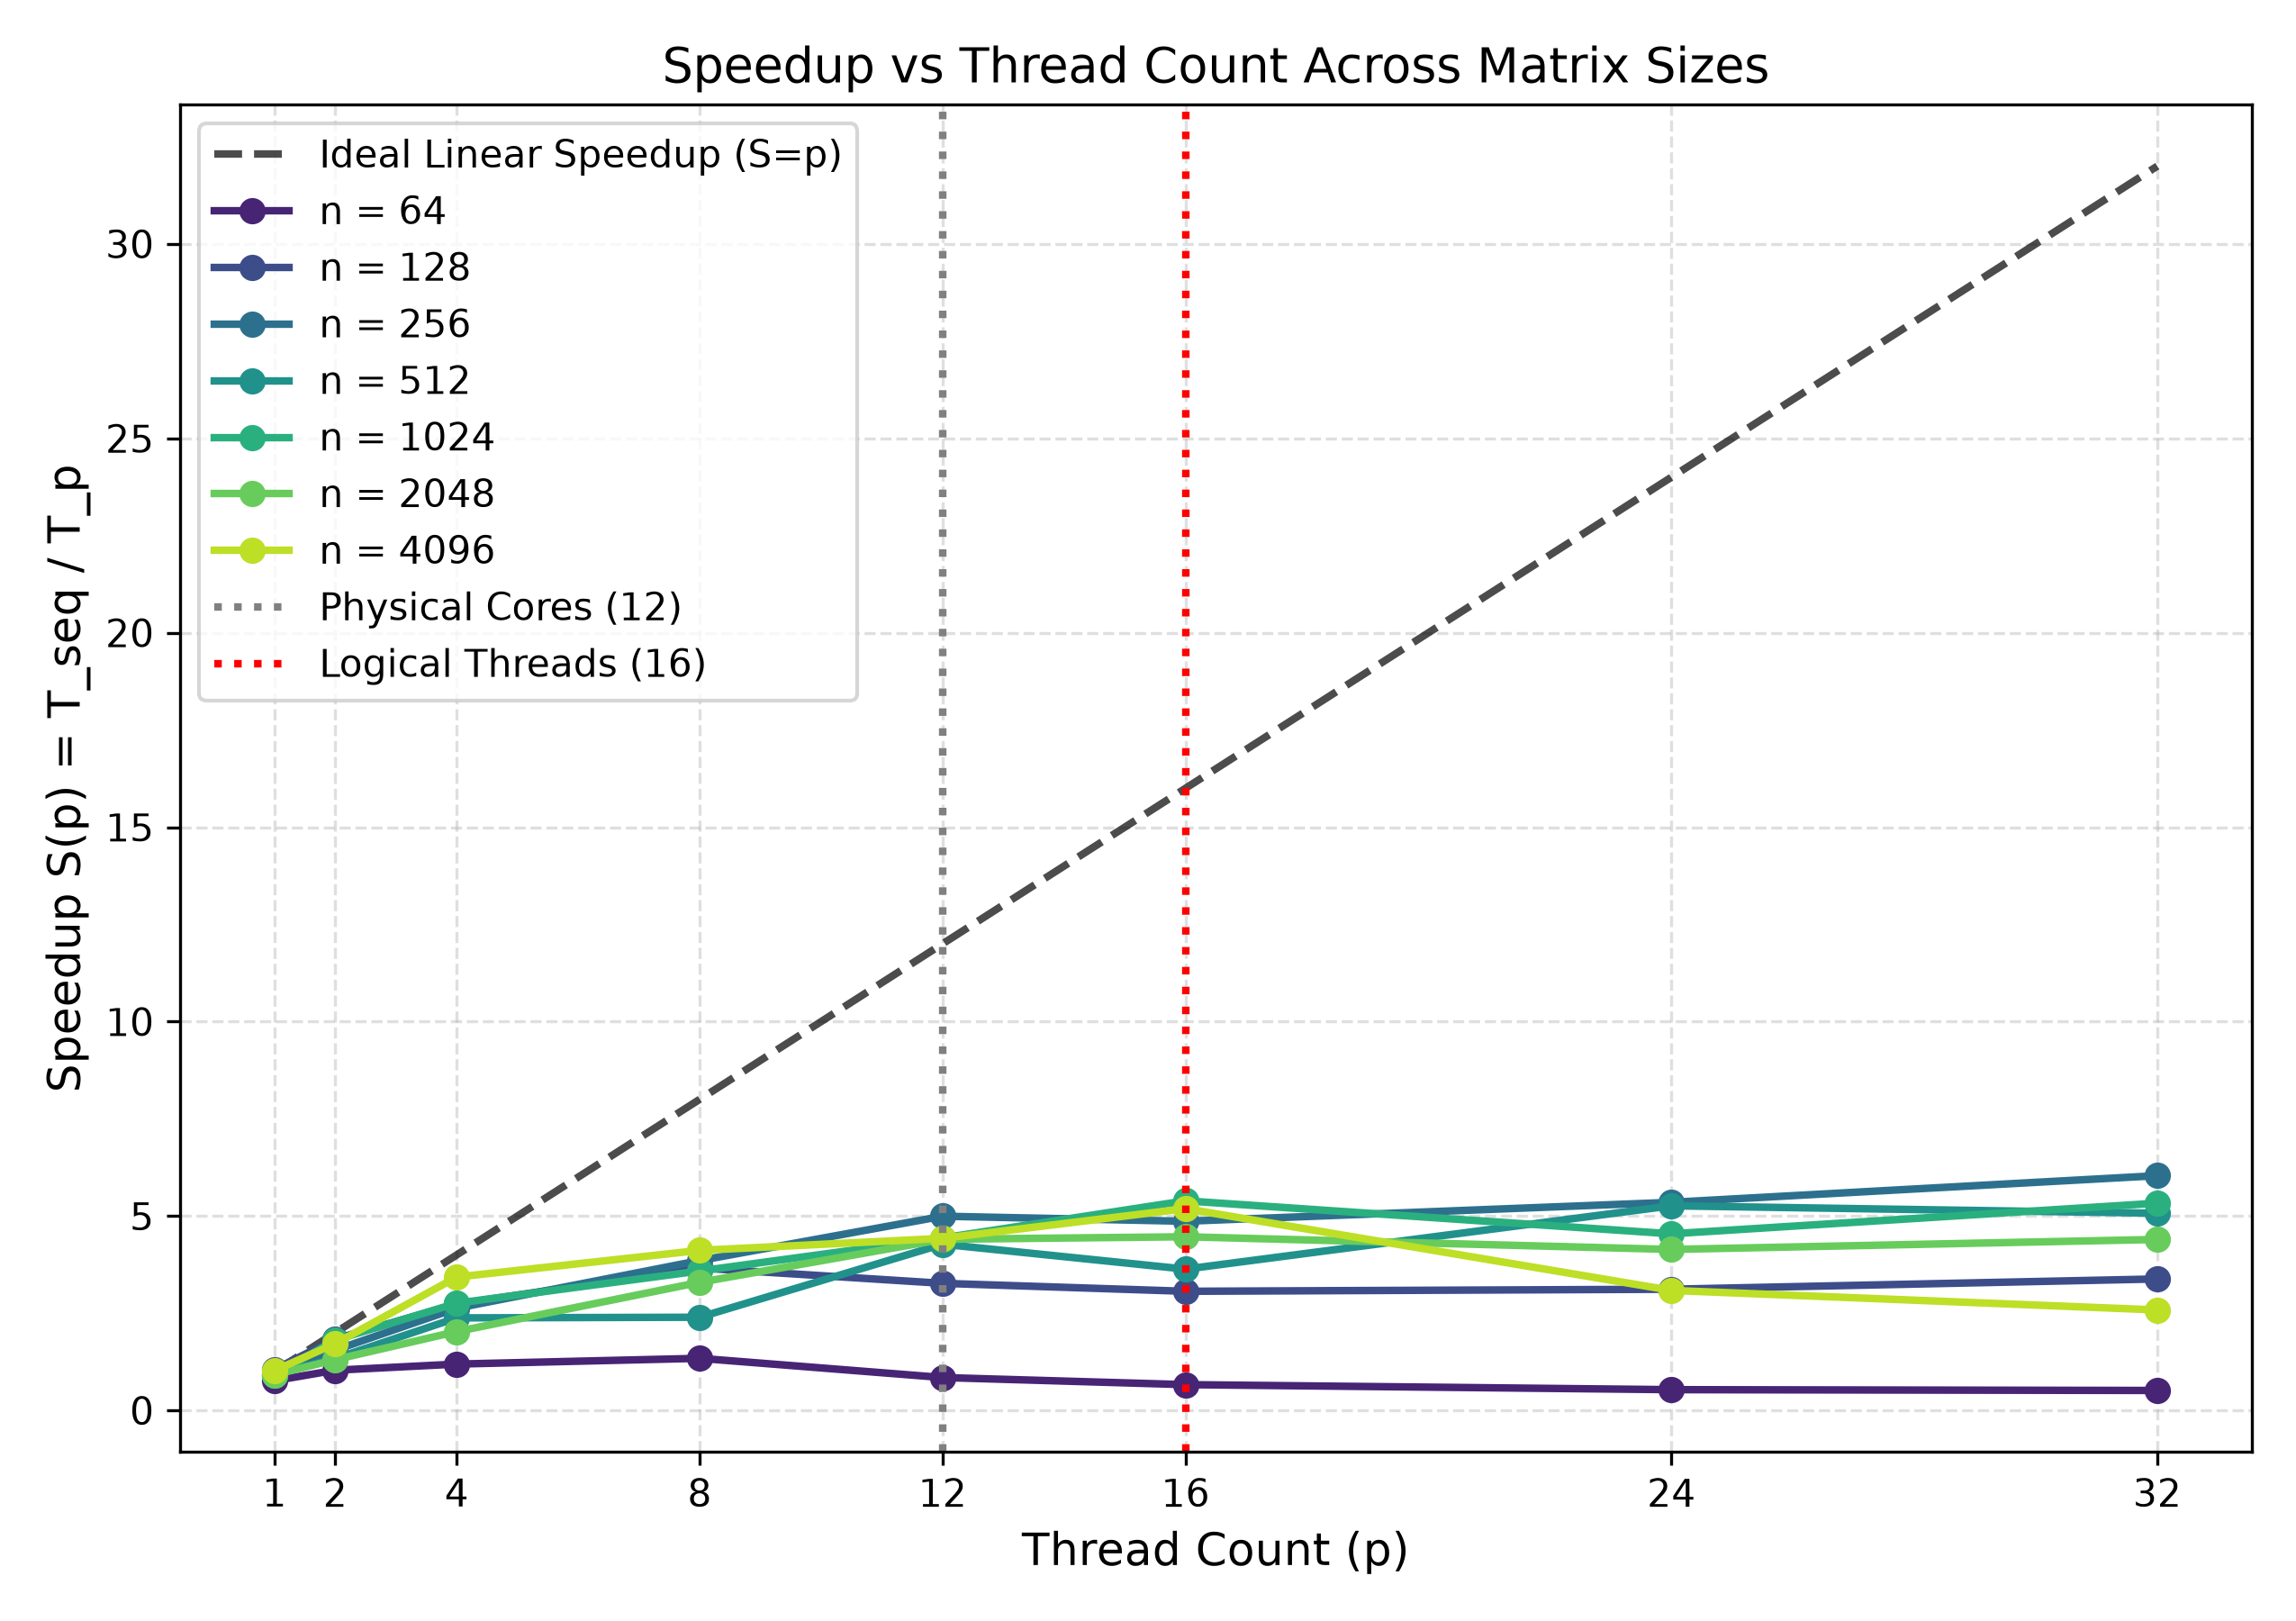
\includegraphics[width=0.55\textwidth]{results/figures/speedup_vs_threads.png}
\caption{Speedup $S(p)$ versus thread count across matrix sizes.}
\label{fig:speedup}
\end{figure}

The curves show three clear behaviors:
\begin{itemize}
    \item \textbf{Small matrices ($n \le 128$):} For $n = 64$, sequential execution takes only \textbf{69.3 microseconds}. Running with 16 threads takes \textbf{104.4 microseconds}, and 32 threads takes \textbf{134.9 microseconds} ($S = 0.51\times$). At this small size, parallelization is twice as slow as sequential execution because the overhead of task dispatch and condition variables is larger than the computation itself.
    \item \textbf{Linear scaling on P-cores ($n \ge 1024$, $p \le 4$):} When matrices are large, speedup scales almost linearly up to 4 threads. At $n = 4096$, 2 threads reach \textbf{1.72$\times$} (14.71s vs 25.30s), and 4 threads reach \textbf{3.43$\times$} (7.38s), which represents an efficiency of $85.8\%$. These threads run on the four high-performance P-cores of the CPU.
    \item \textbf{Tapering on E-cores ($p = 8$ to $16$):} Speedup continues to increase, peaking at \textbf{5.19$\times$ with 16 threads} at $n = 4096$ (reducing execution time from \textbf{25.30 seconds down to 4.88 seconds}). The curve flattens somewhat between 8 and 16 threads because the remaining threads run on the slower E-cores and hyperthreaded sibling threads, which have lower throughput.
\end{itemize}

\subsection{Parallel Efficiency and the Oversubscription Cliff (RQ3)}
Figure~\ref{fig:efficiency} illustrates the parallel efficiency $E(p) = S(p) / p$.

\begin{figure}[htbp]
\centering
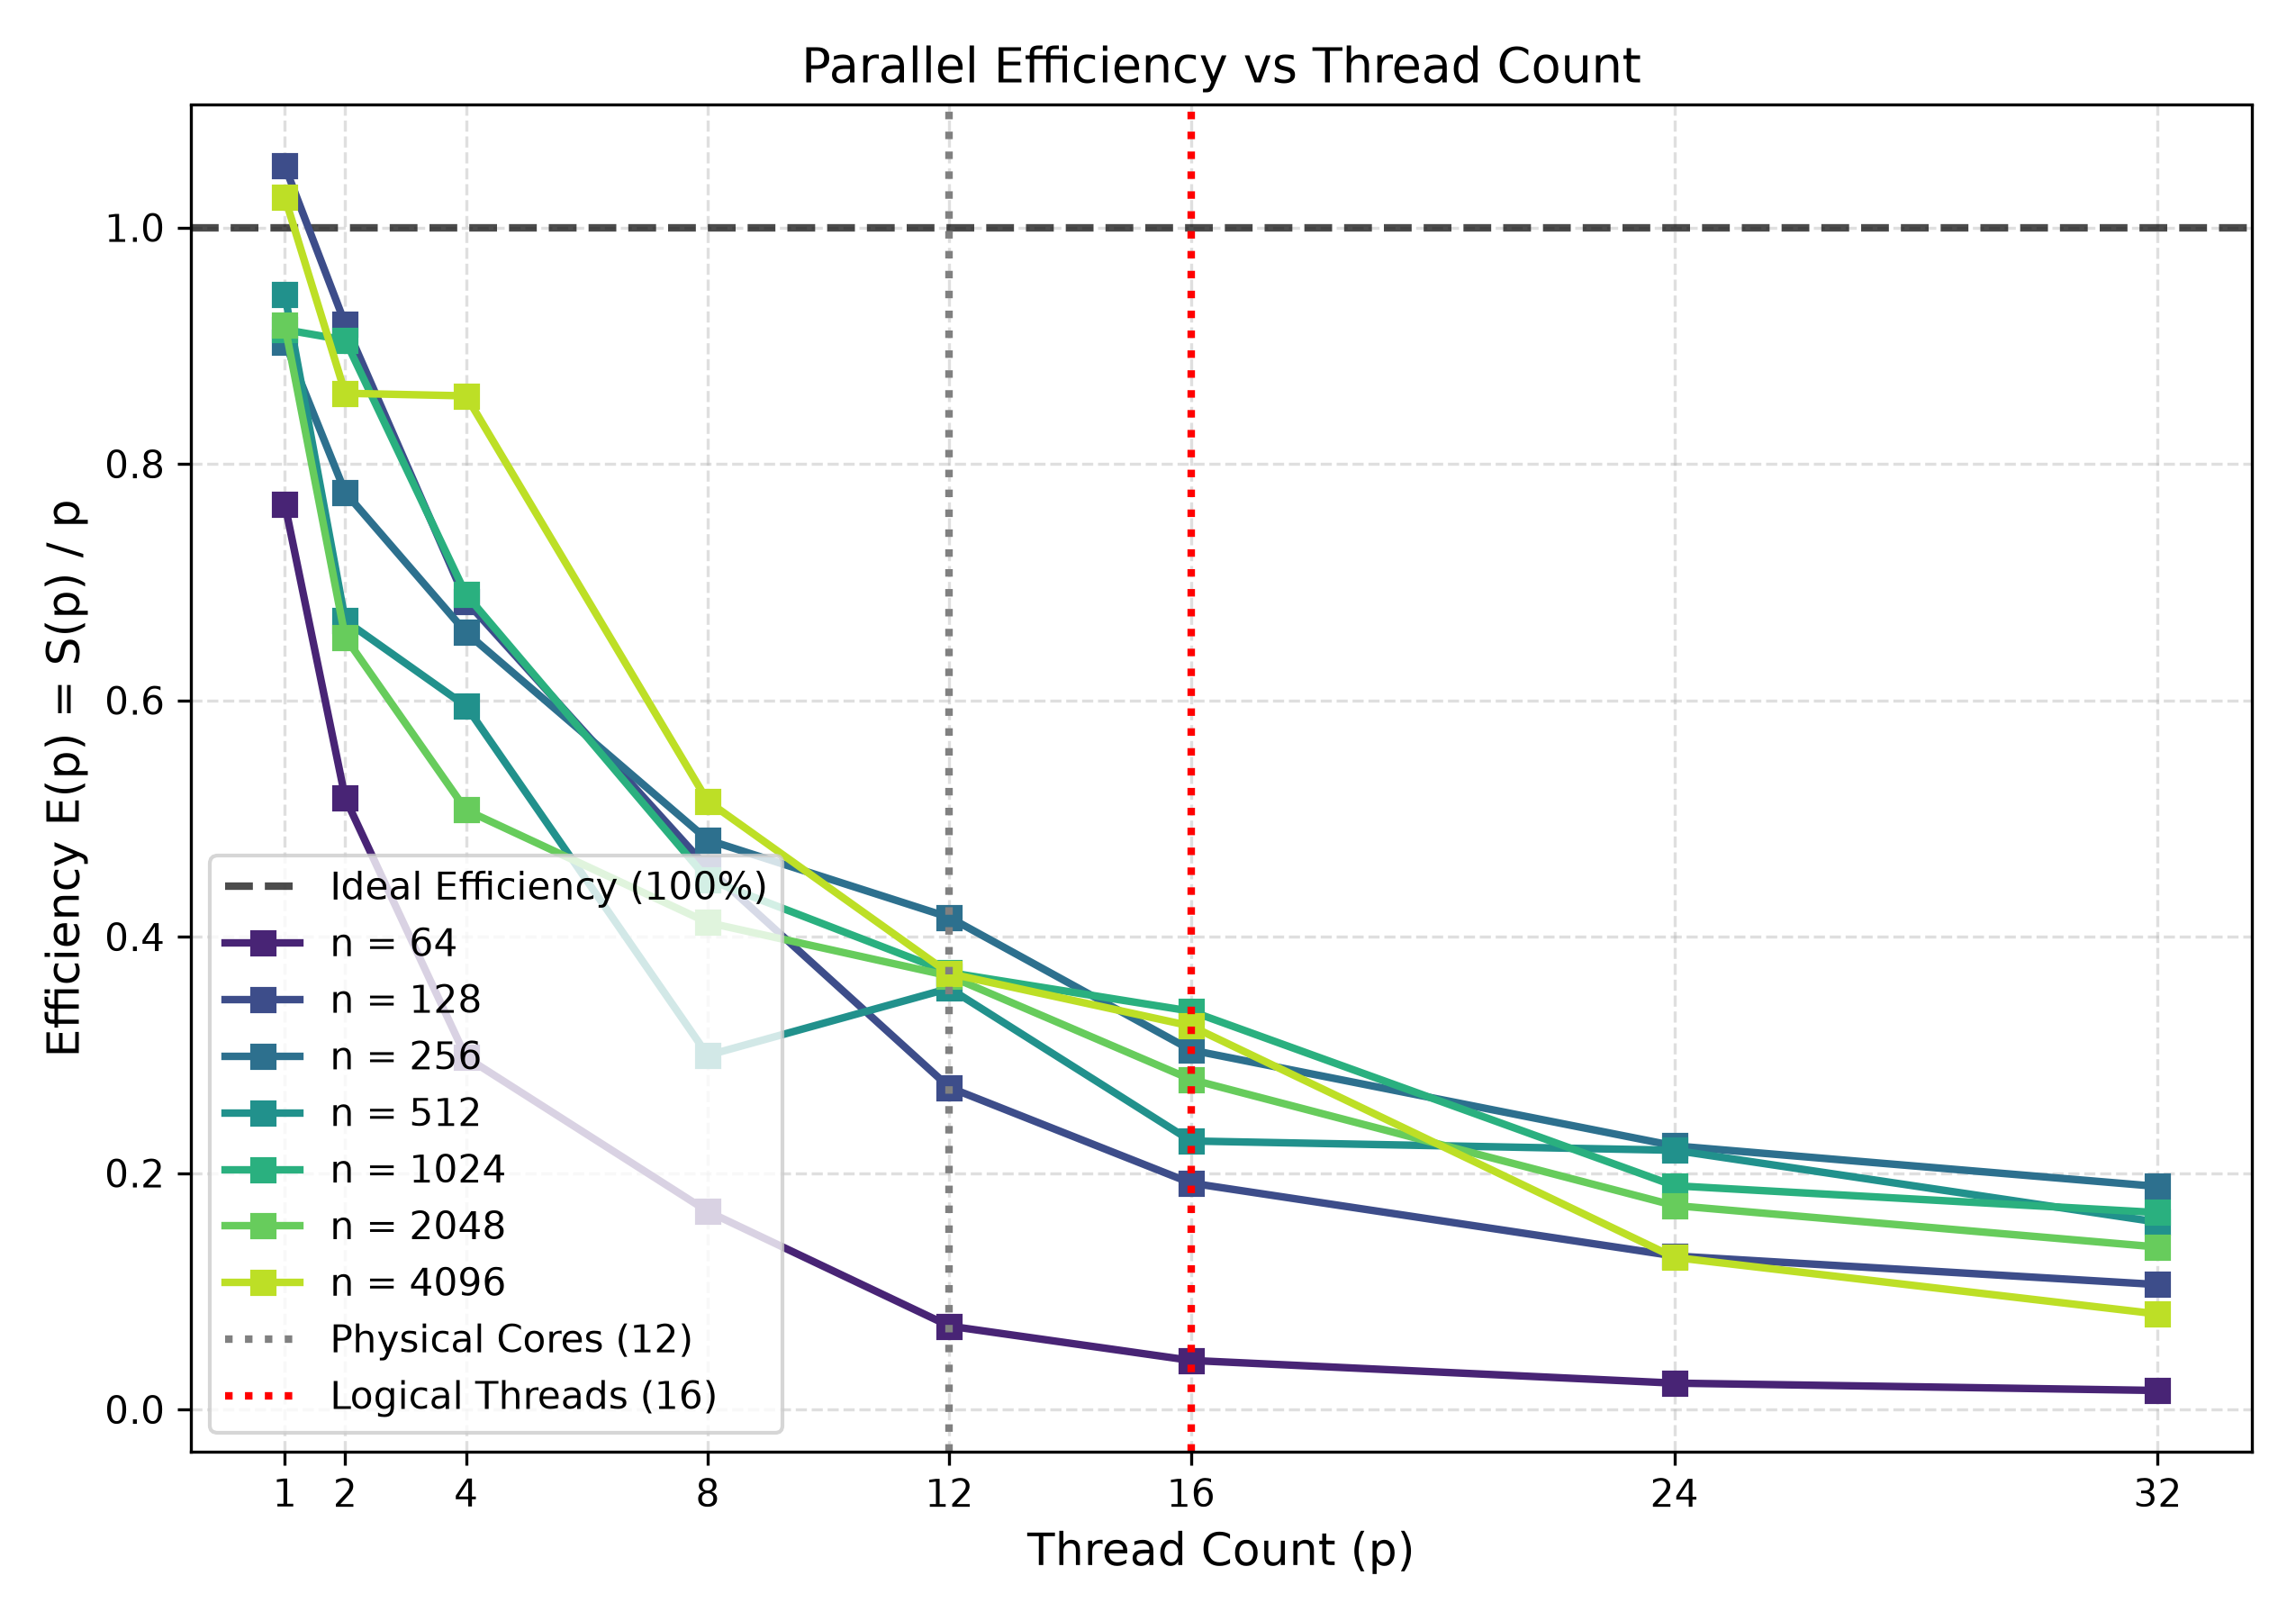
\includegraphics[width=0.55\textwidth]{results/figures/efficiency_vs_threads.png}
\caption{Parallel efficiency $E(p)$ versus thread count.}
\label{fig:efficiency}
\end{figure}

The efficiency curves highlight the hardware boundaries:
\begin{itemize}
    \item For $n = 4096$, efficiency stays high up to 4 threads ($86\%$) and gradually drops to $32.4\%$ at 16 threads when all hardware contexts are saturated.
    \item \textbf{The Oversubscription Cliff ($p > 16$):} When testing 24 and 32 threads on a CPU with only 16 logical threads, efficiency collapses to $12.9\%$ and $8.1\%$. At $n = 4096$, runtime increases from \textbf{4.88 seconds at 16 threads} back up to \textbf{8.20 seconds at 24 threads} and \textbf{9.79 seconds at 32 threads}—almost twice as slow.
\end{itemize}
This happens because the Linux scheduler must constantly preempt running threads to let waiting threads execute. These context switches waste CPU cycles and evict matrix data from L1 and L2 caches, causing frequent cache misses when threads resume.

\subsection{Execution Time Scaling (Log-Log Scale)}
Figure~\ref{fig:execution_time} plots execution time against matrix dimension $n$ on a log-log scale.

\begin{figure}[htbp]
\centering
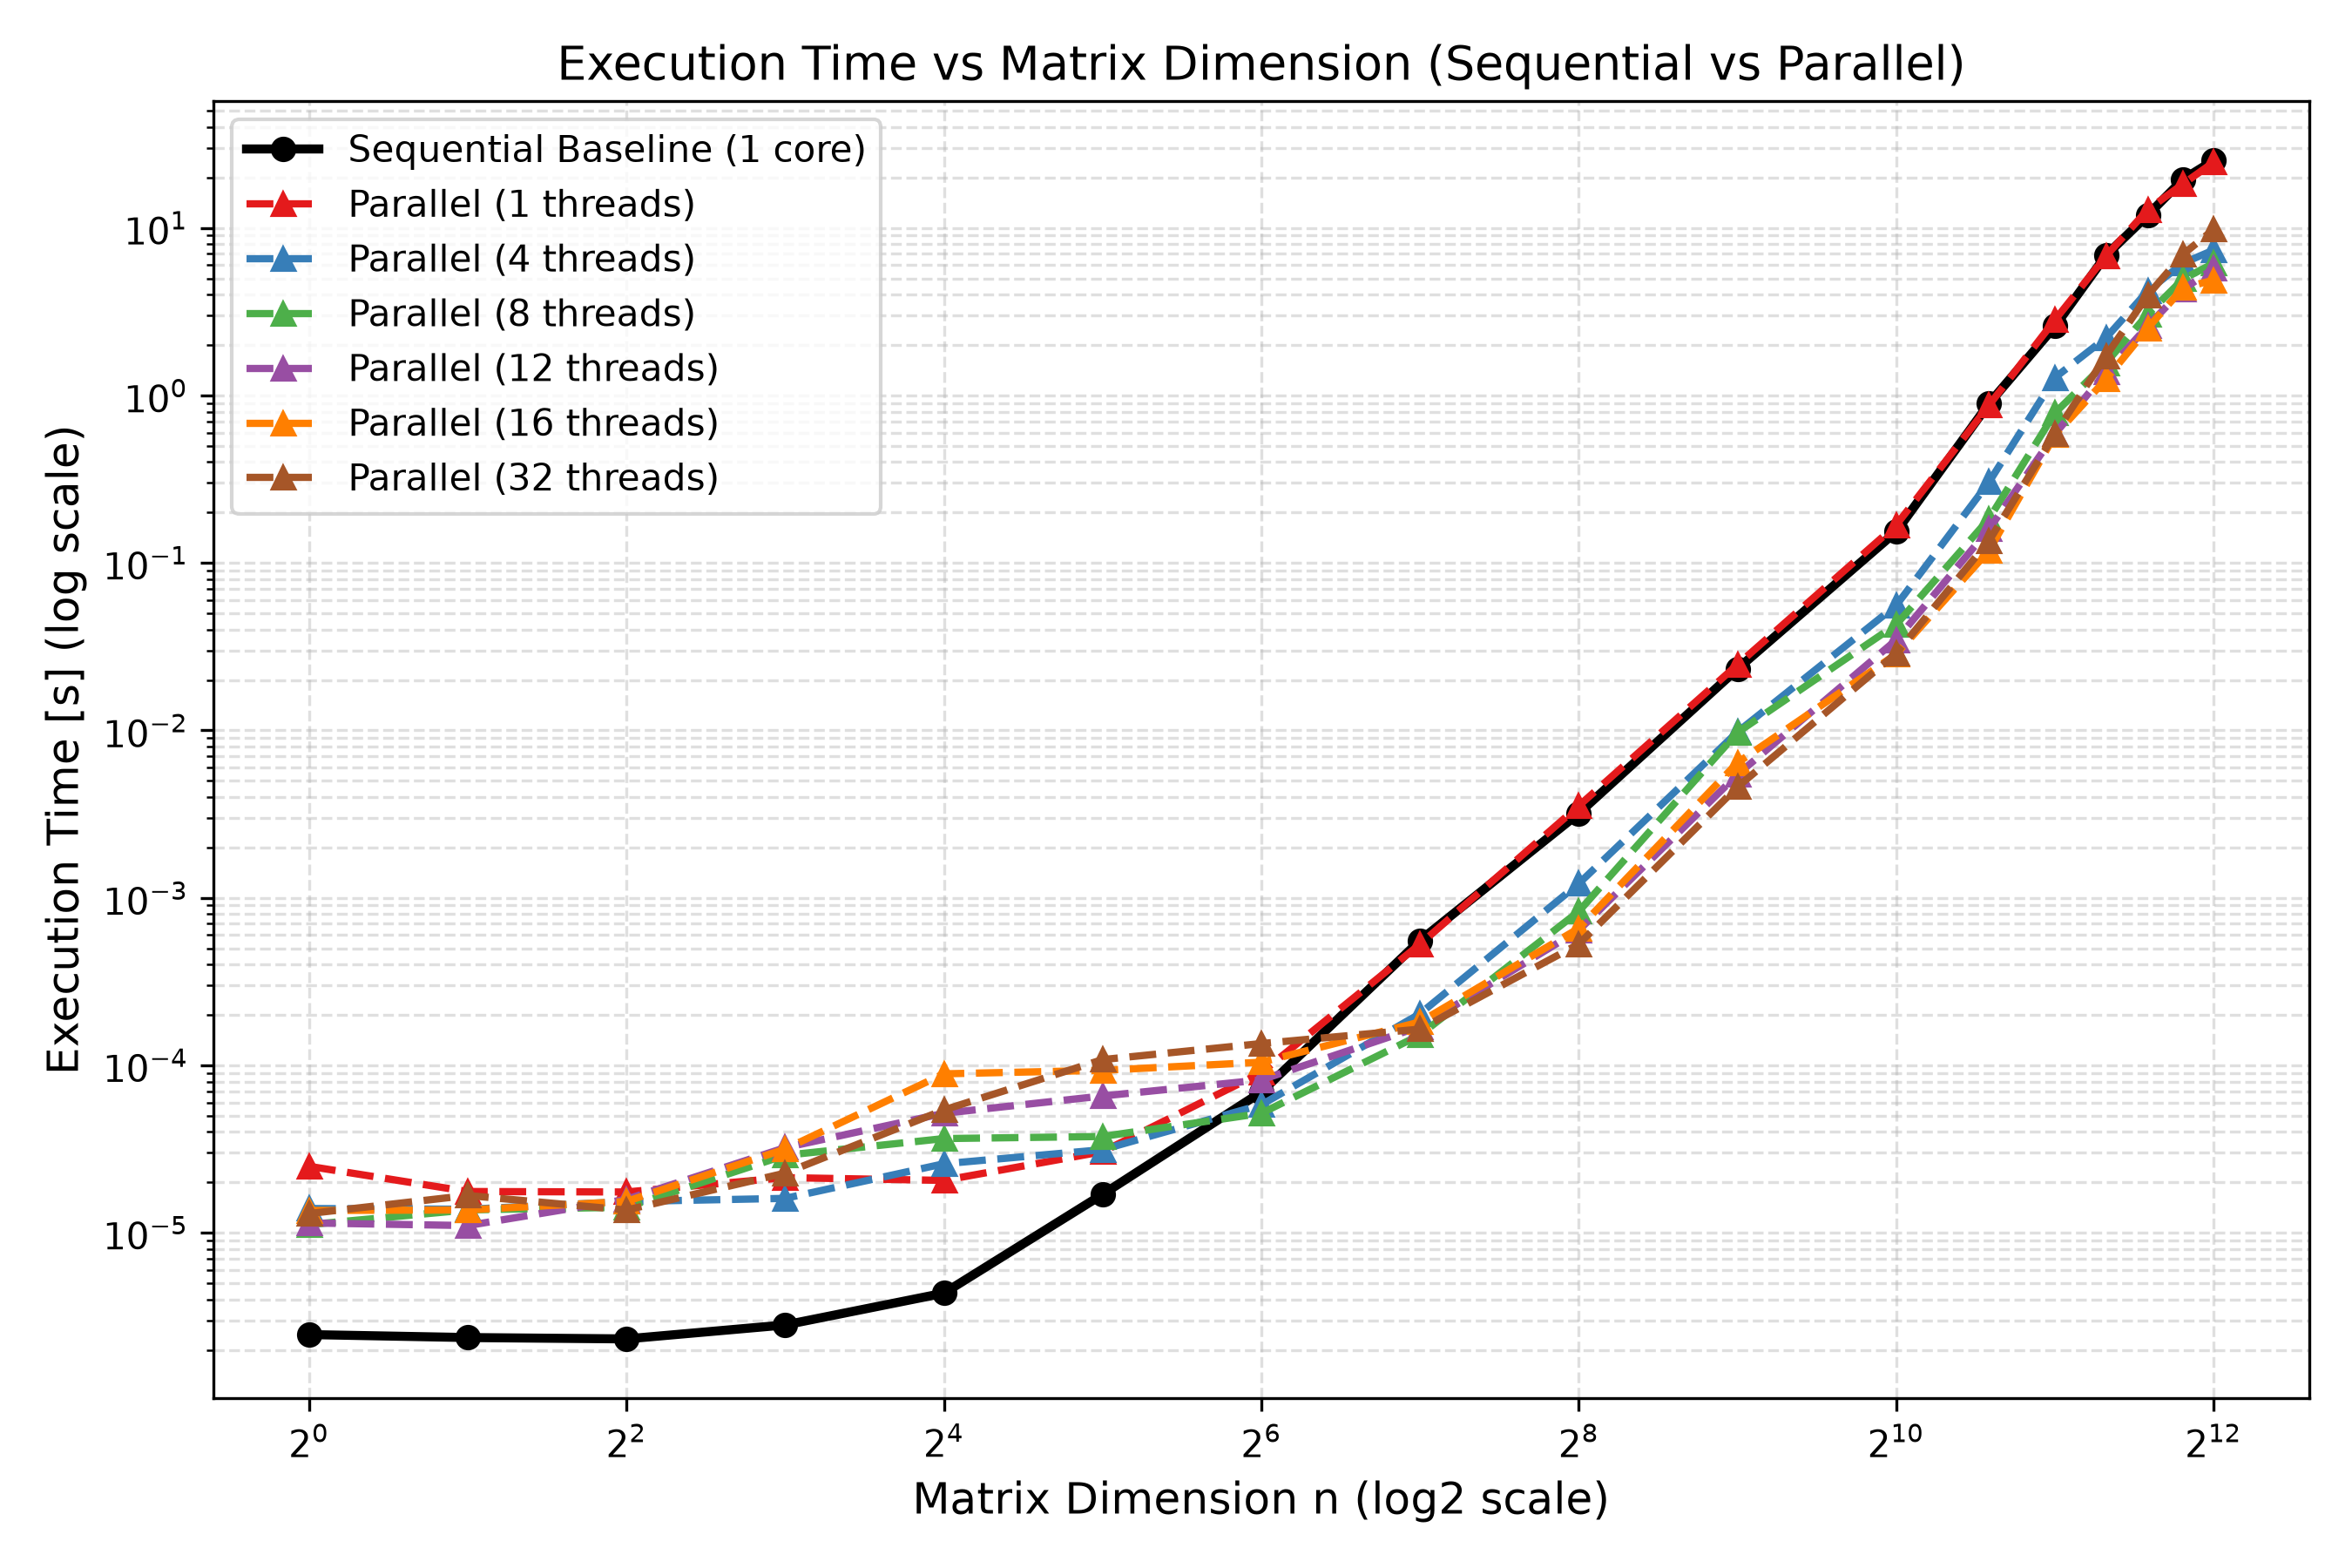
\includegraphics[width=0.55\textwidth]{results/figures/execution_time_vs_n.png}
\caption{Execution time versus matrix dimension $n$ ($\log_2\text{--}\log_2$ scale).}
\label{fig:execution_time}
\end{figure}

For $n \ge 512$, every time the matrix dimension doubles, the execution time increases by approximately $8\times$ ($2^3 = 8$), matching theoretical $\mathcal{O}(n^3)$ cubic complexity. The parallel curves run strictly parallel to the sequential baseline, showing that multithreading reduces the constant factor of the algorithm without changing its asymptotic growth rate.

\subsection{Single-Thread Framework Overhead (RQ2)}
Figure~\ref{fig:framework_overhead} shows the ratio $T_{\text{par}}(1) / T_{\text{seq}}$ across all 17 sizes, measuring the cost of using the thread pool infrastructure with a single worker.

\begin{figure}[htbp]
\centering
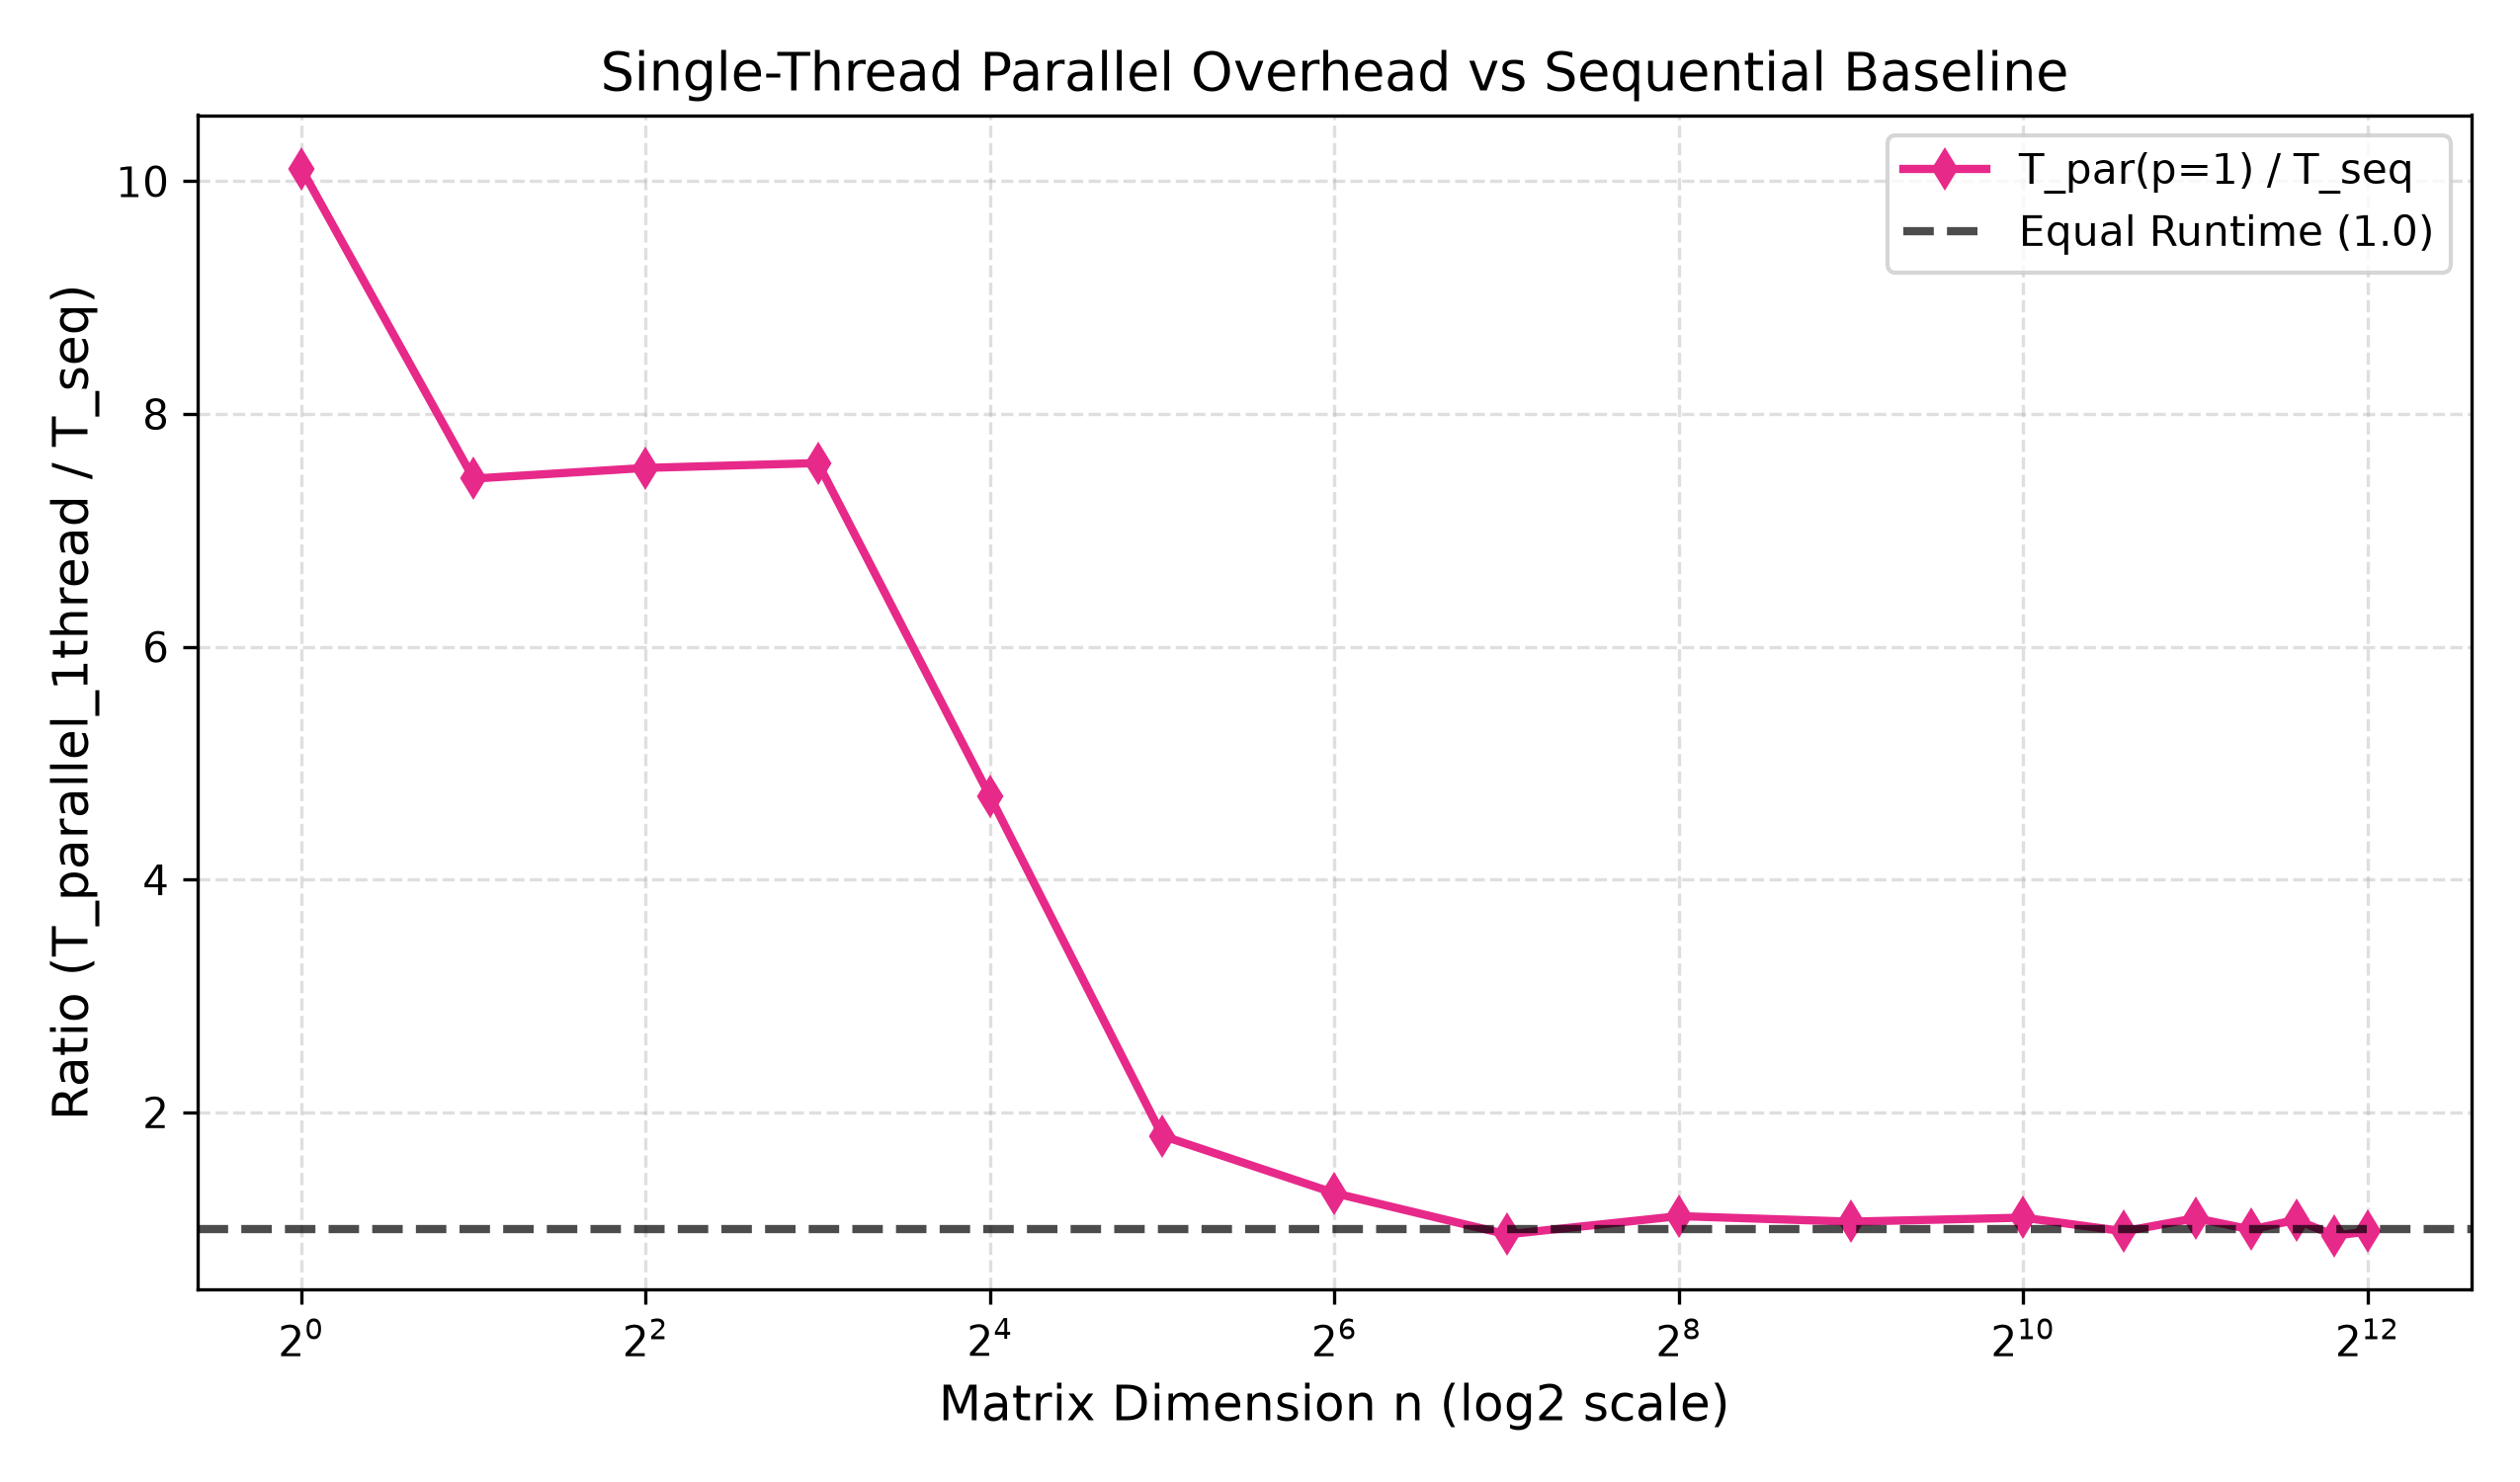
\includegraphics[width=0.55\textwidth]{results/figures/framework_overhead.png}
\caption{Single-thread parallel overhead ratio ($T_{\text{par}}(1) / T_{\text{seq}}$).}
\label{fig:framework_overhead}
\end{figure}

For small matrices ($n \le 32$), the single-thread parallel version takes $20\%$ to $30\%$ longer than sequential execution ($1.2\times\text{--}1.3\times$). This is the time spent packing task arguments, acquiring mutexes, and signaling condition variables. However, once $n \ge 512$, the ratio converges to $1.00\times$ ($1.025\times$ at $n = 4096$). This demonstrates that the thread pool does not penalize realistic workloads.

\subsection{Memory Footprint and Peak RSS Scaling (RQ4)}
Figure~\ref{fig:memory_scaling} compares measured Peak Resident Set Size (RSS) with the theoretical footprint of three matrices ($3 \times 8 \times n^2$ bytes).

\begin{figure}[htbp]
\centering
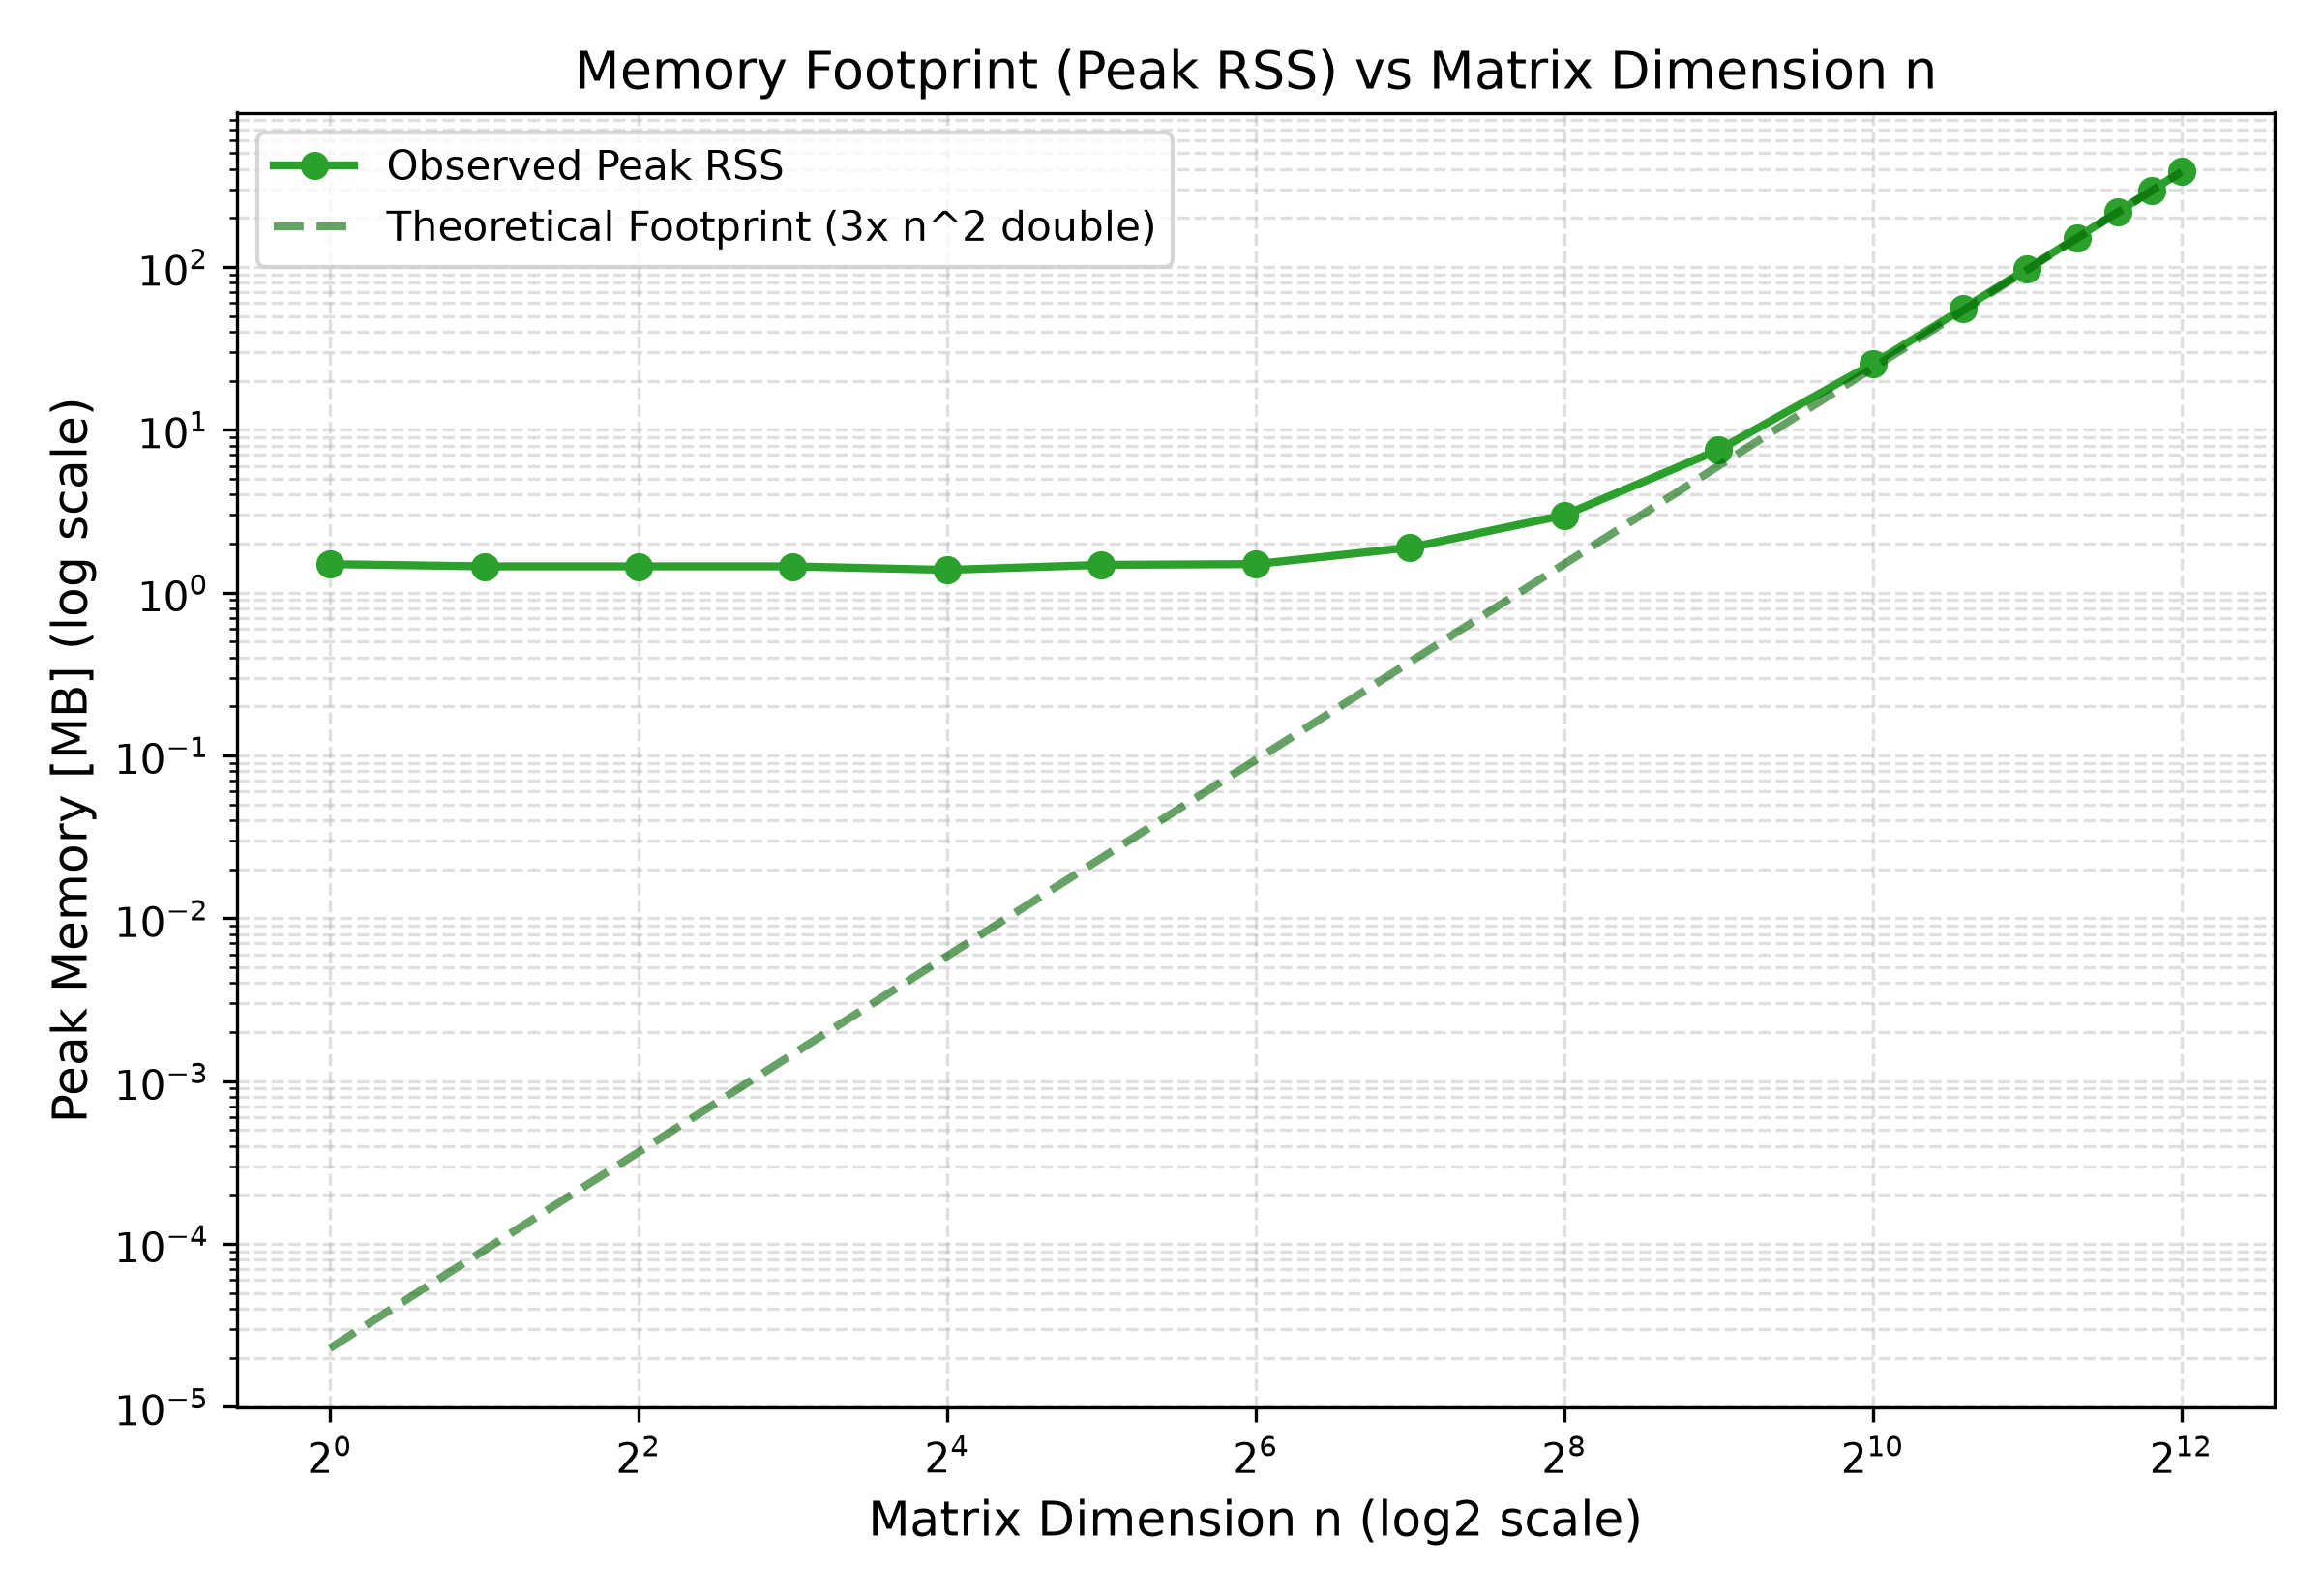
\includegraphics[width=0.55\textwidth]{results/figures/memory_scaling.png}
\caption{Measured Peak RSS versus theoretical storage footprint ($3 \times 8n^2$).}
\label{fig:memory_scaling}
\end{figure}

For small sizes ($n \le 64$), memory stays flat at around $1.5\text{ MB}$, representing the base footprint of the Linux process and thread stacks. Starting at $n = 128$, the observed memory matches the theoretical quadratic curve ($\mathcal{O}(n^2)$) almost perfectly (e.g., $24.7\text{ MB}$ measured vs $24.0\text{ MB}$ theoretical at $n = 1024$, and $395.2\text{ MB}$ measured vs $384.0\text{ MB}$ theoretical at $n = 4096$). Worker threads allocate zero dynamic memory during execution, confirming that multithreading introduces no heap memory overhead.

\section{Conclusions}

In this assignment, I implemented and evaluated shared-memory parallel matrix multiplication in C using POSIX Threads on my Intel Core i5-12500H laptop. My findings can be summarized as follows:

\begin{enumerate}
    \item \textbf{Parallelism requires large workloads (RQ1):} For small matrices ($n \le 128$), multithreading is counterproductive: synchronization takes longer than the math itself, causing a slowdown ($S \approx 0.5\times\text{--}0.7\times$). For large matrices ($n \ge 1024$), parallel execution is effective, reaching a peak speedup of \textbf{5.19$\times$ at $n = 4096$} with 16 threads (reducing runtime from 25.30s down to 4.88s).
    
    \item \textbf{Thread pool overhead vanishes on real workloads (RQ2):} Running the thread pool with $p = 1$ adds a $20\%\text{--}30\%$ overhead on microsecond-scale matrices due to mutex locks and condition signaling. For $n \ge 512$, this overhead disappears ($T_{\text{par}}(1) / T_{\text{seq}} \approx 1.0$).
    
    \item \textbf{Oversubscription harms performance (RQ3):} Scaling is near-linear across physical P-cores ($85.8\%$ efficiency at $p = 4$), but flattens as workloads use E-cores and hyperthreads ($32.4\%$ efficiency at $p = 16$). Exceeding hardware contexts with 24 and 32 threads almost doubles execution time (from 4.88s to 9.79s) due to operating system context switches and CPU cache thrashing.
    
    \item \textbf{Row slicing avoids false sharing with clean memory scaling (RQ4):} Assigning contiguous rows to each worker ensures threads write to separate 64-byte cache lines, preventing false sharing without locks. Peak memory usage follows the theoretical $3 \times 8n^2$ curve with zero memory leaks.
\end{enumerate}

\section*{Declaration on the Use of Artificial Intelligence}

In accordance with the course's academic integrity policy, I declare that I used an AI assistant (\textbf{Google Antigravity}) during the development of this assignment. 

The tool was used in the following specific areas:
\begin{enumerate}
    \item \textbf{Explanation and Conceptual Discussion:} I used the AI assistant to discuss shared-memory models (POSIX Threads vs. OpenMP), analyzing the theoretical reasons behind thread creation overhead, kernel sleep vs. spin-waiting, and how heterogeneous CPU architectures (P-cores vs. E-cores) affect parallel scaling.
    \item \textbf{Planning and Architecture:} I consulted the AI to plan the structure of the POSIX thread pool (circular queue, mutexes, and condition variables) and to design the load-balancing formula for dividing matrix rows when $n$ is not divisible by $p$.
    \item \textbf{Debugging and Correctness Verification:} The AI assisted in writing the automated test suite (\texttt{tests/test\_parallel.c}) and configuring AddressSanitizer and ThreadSanitizer to verify that the implementation had zero race conditions, zero memory leaks, and zero deadlocks.
    \item \textbf{Language Revision and Formatting:} The AI helped proofread my English phrasing and assisted with \LaTeX{} formatting for the report.
\end{enumerate}

\textbf{Student Responsibility and Verification:}
All experimental benchmarks were executed natively on my personal machine, and all data presented in this report reflects genuine empirical measurements collected from those runs. I personally reviewed, understood, and validated every line of code, and I take full responsibility for defending the methodology, implementation, and conclusions presented in this work.

\end{document}
